\documentclass{article}

\usepackage[spanish]{babel}
\usepackage[utf8]{inputenc}
\usepackage{siunitx} % Provides the \SI{}{} and \si{} command for typesetting SI units
\usepackage{graphicx} % Required for the inclusion of images
\usepackage{amsmath} % Required for some math elements 
\usepackage{hyperref}
\usepackage{amsmath}
\usepackage{listings}
\usepackage{xcolor}
\usepackage{courier}
\usepackage[margin=1.2in]{geometry}
\usepackage{changepage}
\usepackage{titlesec}
\usepackage{wrapfig}
\usepackage{colortbl}
\usepackage{booktabs}
\usepackage{multirow}

\definecolor{codegreen}{rgb}{0,0.6,0}
\definecolor{codegray}{rgb}{0.5,0.5,0.5}
\definecolor{codepurple}{rgb}{0.58,0,0.82}
\definecolor{backcolour}{rgb}{0.95,0.95,0.92}

\lstdefinestyle{mystyle}{
    backgroundcolor=\color{backcolour},   
    commentstyle=\color{codegreen},
    keywordstyle=\color{magenta},
    numberstyle=\tiny\color{codegray},
    stringstyle=\color{codepurple},
    basicstyle=\ttfamily\footnotesize,
    breakatwhitespace=false,         
    captionpos=b,                    
    keepspaces=true,                 
    numbers=left,                    
    numbersep=5pt,                  
    showspaces=false,                
    showstringspaces=false,
    showtabs=false,                  
    tabsize=2
}
\lstset{language=Python, 
        basicstyle=\ttfamily\small, 
        keywordstyle=\color{keywords},
        commentstyle=\color{comments},
        stringstyle=\color{red},
        showstringspaces=false,
        identifierstyle=\color{codepurple},
        keywords=[2]{pow},
        keywordstyle=[2]{\color{orange}},
}

\lstset{style=mystyle}

\setlength\parindent{0pt} % Removes all indentation from paragraphs

\renewcommand{\labelenumi}{\alph{enumi}.} % Make numbering in the enumerate environment by letter rather than number (e.g. section 6)

\title{\textrm{\textbf{\LARGE Análisis del movimiento \\ de un objeto en un \\ plano inclinado}}} % Title

\author{Víctor Mira Ramírez} % Author name

\date{\today} % Date for the report

\begin{document}

\maketitle % Insert the title, author and date

\begin{center}
\begin{tabular}{l r}

Profesor: & Carlos Sabater Piqueres\\
Grupo: & Grupo III \\
Lugar: & Universidad de Alicante
\end{tabular}
\end{center}

\hfill \break \\

\tableofcontents

%----------------------------------------------------------------------------------------
%	SECTION 1
%----------------------------------------------------------------------------------------
\pagebreak

\begin{abstract}
En esta práctica describiremos el movimiento de diferentes objetos sobre planos inclinados. Se harán medidas de tiempos de caída de objetos de distintas formas, masas y materiales.También estudiaremos los conceptos de dinámica y cinemática, caracterizando los coeficientes de fricción del sistema además de la conservación de la energía mecánica. Por último, se estudiará el movimiento de cilindros que caen por un plano inclinado.
\end{abstract}

\section{Introducción}
Con el material suministrado se deberán comprobar las ecuaciones de movimiento del sistema a estudiar y la ley de conservación de la energía.
Se caracterizarán los coeficientes de rozamiento estático y dinámico entre los materiales suministrados. Se discutirá el efecto de la masa y la forma el objeto sobre la fuerza de rozamiento.
Para todos estos cálculos necesitaremos usar una serie de ecuaciones:

\begin{equation}\label{eq:varianza}
    \centering
    S_x = \sqrt{\sum_{j=1}^{N}\frac{\left(x_j - \bar{x}\right)^2}{N-1}} \quad \Rightarrow \quad
    \Delta_{est} = \frac{S_x}{\sqrt{N}}
\end{equation}

\vspace{0.3cm}

\begin{equation}\label{eq:derivadas parciales}
    \centering
    \triangle{V} = \sqrt{\left(\frac{\partial{V}}{\partial{x}}\right)^2 \triangle{x}^2 + \left(\frac{\partial{V}}{\partial{y}}\right)^2 \triangle{y}^2 + \left(\frac{\partial{V}}{\partial{z}}\right)^2 \triangle{z}^2 }
\end{equation}

\vspace{0.3cm}

\begin{equation}\label{eq:graf}
    \centering
    y = a\cdot{x} + b
\end{equation}

\vspace{0.3cm}

\begin{equation}\label{eq:minscuad}
    \centering
    a_0 = \frac{N\sum x_i\cdot{y_i} - \sum x_i\cdot{y_i}}{N\sum {x_i}^2 - \left(\sum x_i \right)^2} \quad \Rightarrow \quad
    b_0 = \frac{\left(\sum x_i \right)^2\cdot{y_i} - \sum x_i\cdot\sum x_i\cdot{y_i}}{N\sum {x_i}^2 - \left(\sum x_i \right)^2}
\end{equation}

\vspace{0.3cm}

\begin{equation}\label{eq:errorminscuad}
    \centering
    \sigma_a = \sqrt{\frac{{\chi_N}^2}{N\cdot{Var(x)}}}
    \quad \Rightarrow \quad
    \sigma_b = \sqrt{\frac{{\chi_N}^2\cdot{\sum_(i=1)^(N) {x_i}^2}}{N\cdot{Var(x)}}}
\end{equation}

\vspace{0.3cm}

\begin{equation}\label{eq:newton}
    \centering
    F = m \cdot a
\end{equation}

\vspace{0.3cm}

La ecuación \eqref{eq:varianza} se usará para la obtención del error estadístico de las diferentes medidas obtenidas del programa tracker y los videos grabados. Por otro lado, \eqref{eq:derivadas parciales} nos servirá para propagación de errores, y \eqref{eq:graf} nos será útil una vez linealizada la gráfica, donde a es la pendiente y b la ordenada en el origen. Por último, la ecuación \eqref{eq:minscuad} es la de ajustes por mínimos cuadrados, útil para linealizar, junto con sus errores \eqref{eq:errorminscuad}. La ecuación \eqref{eq:newton} es la segunda ley de Newton.

\clearpage

\section{Diagramas y formulaciones matemáticas}

El siguiente diagrama muestra un cuerpo sobre un plano inclinado y las fuerzas que actúan sobre él. 

\begin{figure}[h]
\centering
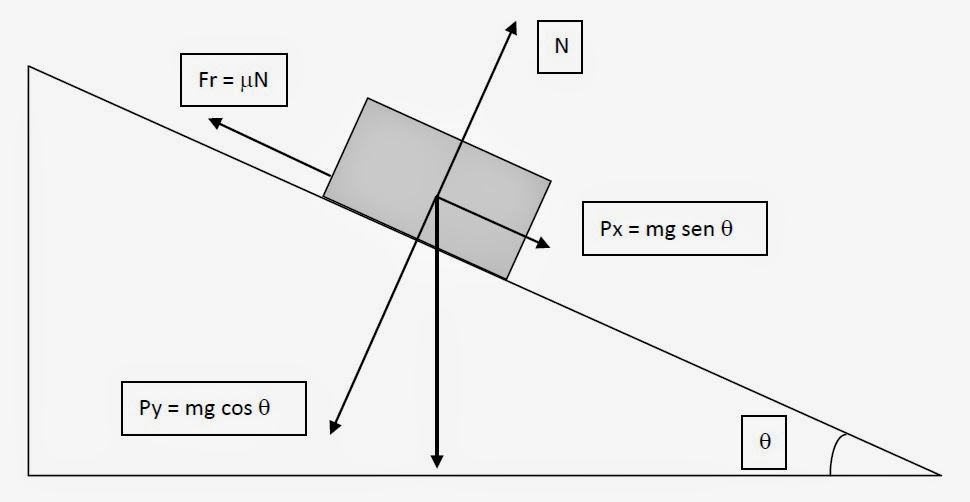
\includegraphics[width=.75\textwidth]{fotos/plano inclinado.jpg}
\end{figure}

Podemos ver que aunque el peso está alineado con los ejes, solo su componente multiplicada por $\sin{\theta}$ acelera al cuerpo, mientras que la componente multiplicada por $\cos{\theta}$ provocará una fuerza normal, $N$, que, multiplicada por el coeficiente de rozamiento entre el material del cuerpo y el material del plano, nos generará una fuerza de rozamiento en sentido opuesto al movimiento.\\\\


\subsection{Cuerpo estático}
Para obtener el coeficiente de rozamiento estático aplicaremos la Segunda Ley de Newton, \eqref{eq:newton} $F = m \cdot a$, (sumatorio de las fuerzas aplicadas sobre un cuerpo es igual a su masa multiplicada por la aceleración). \\ En nuestro caso, tenemos dos fuerzas que se oponen, la componente del peso que es paralela al plano inclinado y la fuerza de rozamiento $P_x - F_r = m \cdot a$. Pero en nuestro caso, el cuerpo todavía no ha empezado a moverse, y por tanto la aceleración será nula $a = 0$. Así, la formula quedará como $P_x - F_r = 0$ o, escrito de otra forma:
\[ \boxed{P_x = F_r} \]
En este instante inicial, la fuerza de rozamiento será máxima y, utilizando las fórmulas:
\[ P_x = m \cdot g \sin{\theta} \]
\[ N = P_y = m \cdot g \cos{\theta} \]
\[ F_r = \mu_e \cdot N\]
y igualándolas entre sí, obtenemos
\[ m \cdot g \cdot \sin{\theta} = \mu_e \cdot m \cdot g \cdot \cos{\theta}\]
\[ \textbf{\large{\boxed{\mu_e = \tg{\theta}}}} \]

\clearpage
\subsection{Cuerpo dinámico}
El coeficiente de rozamiento dinámico describe la oposición al movimiento que dos cuerpos en contacto experimentan en sus superficies. Dicho coeficiente es característico de cada pareja de materiales que escojamos, y dependerá de otros factores como por ejemplo la temperatura ambiente. \\ \\
Para obtener el coeficiente de rozamiento dinámico necesitaremos conocer la aceleración del cuerpo que se desliza por nuestro plano inclinado, que tendrá que tener un ángulo mayor al ángulo límite del coeficiente de rozamiento estático. \\\\
Como ya hemos visto en el apartado del coeficiente estático, $P_x - F_r = m \cdot a$, pero esta vez la aceleración no será nula.\\
\[ P_x - F_r = m \cdot a \]
\[ m \cdot g \cdot \sin{\theta} - \mu_d \cdot m \cdot g \cdot \cos{\theta} = m \cdot a\]\\
Aquí podemos despejar la masa a ambos lados y vemos que se va, quedándonos:\\\\
\[ \sin{\theta} - \mu_d \cdot \cos{\theta} = \frac{a}{g}\]
\[ \mu_d \cdot \cos{\theta} - \sin{\theta} = -\frac{a}{g} \]
\[ \mu_d \cdot \cos{\theta} = \sin{\theta} - \frac{a}{g} \]\\
Finalmente, despejamos el coeficiente de rozamiento dinámico:\\
\[ \textbf{\large{\boxed{\mu_d = \frac{\sin{\theta}-\frac{a}{g}}{\cos{\theta}}}}} \]


%-----------------{\theta}-----------------------------------------------------------------------
%	SECTION 4
%----------------------------------------------------------------------------------------
\clearpage

\section{Desarrollo experimental}

\paragraph{Material proporcionado}\mbox{}
    \begin{tabular}{ll}
        Plano inclinado& \\
        Plancha de goma& \\
        Cuerpo de madera y aluminio& \\
        Pesa& \\
        Programa "Tracker"& \\
        Teléfono móvil& \\
        Cuerpos cilíndricos de aluminio y PVC& \\
    \end{tabular}    
    
\paragraph{Otras medidas}\mbox{}
    \begin{tabular}{ll}
        Longitud del plano inclinado& $0.6\,\pm\  0.1\,m$\\
        Masa del cuerpo de madera&
        $0.07130\,\pm\ 0.00001\,kg$\\
        Masa del cuerpo de aluminio&
        $0,20294\, \pm\ 0.00001\,kg$\\
        Masa de la pesa&
        $0,05000\, \pm\ 0.00001\,kg$
    \end{tabular}\\\\

\subsection{Preparación}
El primer paso antes de empezar es limpiar concienzudamente tanto los cuerpos como la superficie, tratando de eliminar cualquier residuo o imperfección que haya podido quedar en la misma. Seguidamente, usaremos una balanza para obtener un valor para la masa del cuerpo de madera y el cuerpo de aluminio, así como la pesa que se nos proporciona. Mediremos también la longitud del plano inclinado y realizaremos una marca en lo más alto del mismo y al final. Gracias a estas marcas nos aseguraremos de que los cuerpos son soltados desde la misma altura en todas las ocasiones.\\\\

\begin{figure}[h]
\centering
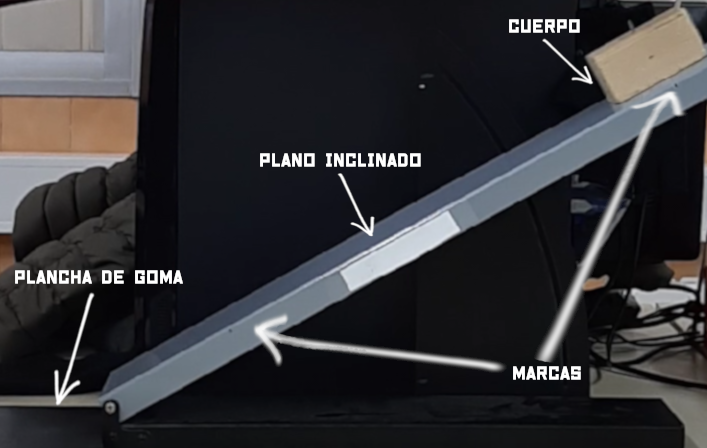
\includegraphics[width=.75\textwidth]{fotos/plano.png}
\end{figure}

\clearpage
\subsection{Coeficiente estático}
Para calcular el coeficiente de rozamiento estático, realizamos 5 medidas diferentes para varios ángulos iniciales y con ambos cuerpos. \\\\ 
Comenzamos pues a tomar medidas, colocamos uno de los cuerpos en la marca más alta, y una plancha de goma al final del plano inclinado para absorber los golpes. Poco a poco iremos aumentando el ángulo del plano inclinado hasta que el cuerpo comience a caer. Anotaremos el ángulo y volvemos a empezar. Repetimos esta operación cinco veces con cada cuerpo con y sin pesa. Estudiaremos la existencia de dispersión en la medida \\\\ Este será el ángulo límite en el cual $P_x$ vence a $F_r$ estática y el cuerpo empieza a caer. Obtendremos así, y gracias al desarrollo matemático explicado en el apartado 2, el coeficiente de rozamiento estático de ambos cuerpos y el aluminio del cual está hecho el plano inclinado.\\\\

\subsection{Coeficiente dinámico}
De forma similar al estático, realizaremos otras 5 medidas. Esta vez serán 5 vídeos grabados con móviles de los cuales, una vez pasados al ordenador, obtendremos una caracterización de la posición en función al tiempo.\\\\
El primer paso es asegurarse de que tanto la superficie como los cuerpos están debidamente limpios. Una vez limpio, escogeremos un ángulo inicial superior al obtenido en el apartado de coeficiente estático. De esta forma nos aseguraremos de que el cuerpo caerá por el plano para ángulos mayores a el escogido. \\\\ Situaremos un teléfono móvil en un trípode frente al plano inclinado dejando en el plano de la cámara todo el plano inclinado y situándose paralelo al mismo. \\ Comenzamos a grabar en el móvil y soltamos el cuerpo desde la marca más alta del plano, y dejamos de grabar cuando llega al final. Aumentamos el ángulo inicial y grabamos otro vídeo. Finalmente obtendremos 5 vídeos para cada cuerpo con y sin pesa. \\\\
Una vez realizadas las medidas, pasaremos los vídeos al ordenador y los abriremos con el programa "Tracker", de donde, una vez situado un punto en cada frame del vídeo donde nuestro cuerpo se situaba, obtenemos unas tablas con los datos de la posición, el tiempo y la velocidad instantánea. \\\\ Gracias a esta tabla y podemos obtener un valor para la aceleración usando fórmulas de cinemática, y con ella, junto con el valor de la masa, podemos obtener el coeficiente de rozamiento dinámico de ambos cuerpos, con y sin la pesa.\\\\ El coeficiente de rozamiento dinámico será menor al estático obtenido en el apartado anterior, y no dependerá de la masa, por lo que será el mismo para cada cuerpo independientemente de si le hayamos añadido o no la pesa. 

\clearpage
\subsection{Conservación de la energía}
Con los datos obtenidos en el programa "Tracker" para el apartado del coeficiente de rozamiento dinámico, podemos caracterizar la evolución de la energía en nuestro experimento. \\\\
Sabemos que la energía cinética se calcula a partir de la expresión:
\[ E_c = \frac{1}{2} m v^2 \]
y que la energía potencial se calcula a partir de la expresión:
\[ E_p = m g h \]
además de que la energía mecánica es la suma de ambas:
\[ E_M = E_c + E_p \]
\\
Pero en nuestro caso, está presente una fuerza disipativa, la fuerza de rozamiento. Por ello, si no la tenemos en cuenta, veremos como la energía mecánica desciende y no se mantiene constante.
Pero sabemos que el trabajo realizado por la fuerza de rozamiento será la diferencia de energía mecánica en el sistema inicial con la final.\\
\[ E_{total} = E_M + W_{F_r} \]
Esta energía total sí se mantendrá constante, ya que tiene en cuenta el trabajo realizado por la fuerza de rozamiento.

\subsection{Sólido Rígido}
Mediremos también la caída de dos cilindros, uno macizo de una masa significativamente mayor al de otro cilindro, esta vez hueco. Ambos tendrán el mismo radio. \\\\ Cuando un cilindro cae por un plano inclinado realiza un movimiento de traslación de su centro de masa y también una rotación de un eje que pasa por ese punto. Las ecuaciones que gobiernan la dinámica de ambos movimientos son: 
\[ -F_r + M g \sin{\beta} = M a\]
\[ F_r r = I \alpha\]
donde $F_r$ es la fuerza de rozamiento, $R$ es el radio del cilindro, $M$ es su masa, $I$ su momento de inercia respecto del eje de rotación, $\beta$ es la inclinación del plano, $\alpha$ es la aceleración angular y a la aceleración del centro de masas del cuerpo. Si el movimiento se realiza rodando sin deslizar, debe cumplirse también que:
\[ \alpha R = a\]
En este caso podemos comprobar que debe cumplirse la siguiente ecuación:

\[ g \sin{\beta} = a \left( 1 + \frac{I}{M R^2} \right)\]


\clearpage
\section{Resultados y Discusiones}
    \subsection{Estático}
    Para esta parte de la práctica, tal y como se ha descrito anteriormente, hemos ido subiendo el ángulo poco a poco, con el cuerpo situado en la parte superior del plano inclinado, hasta que este ha empezado a bajar. \\\\Una vez anotados todos los ángulos, realizamos un análisis estadístico para obtener la media 
    \[\bar{X} = \frac{\sum_{i = 1}^n x_i}{n}\] 
    y la varianza
    \[ S_x = \frac{\sum_{j=1}^{n} \left( x_j - \bar{X}\right)^2}{N-1}\]
    y de ahí, el error estadístico.
    \[ E_{est} = \frac{S_x}{\sqrt{N}}\]\\
    
    Añadiéndole a esto el error nominal del propio instrumento de medida y de interacción con el mismo, obtenemos un error para la tabla de ángulos.\\\\ Una vez obtenido el coeficiente estático a partir de la media de los ángulos, podemos propagar el error del ángulo, ya que es el único que afecta en la fórmula del coeficiente estático ($\mu_e = \tg{\theta}$), y por tanto realizando la tangente a los errores obtenidos para los ángulos, obtenemos el error del coeficiente estático. Da la casualidad de que es el mismo valor para todos ellos una vez ajustado, $\pm \ 0.02.$
    
        \begin{figure}[h]
        \centering
        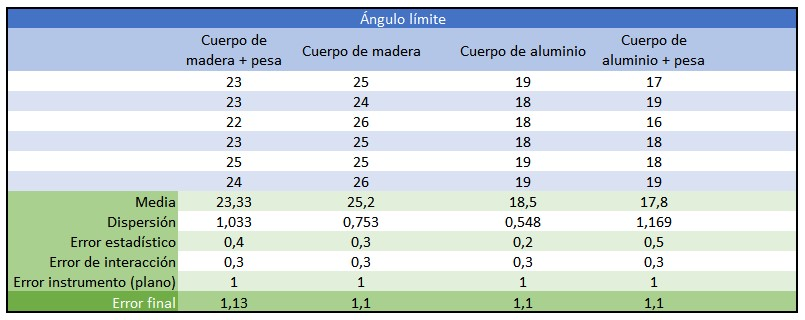
\includegraphics[width=.95\textwidth]{fotos/anglim.jpg}
        \end{figure}
        
        \begin{figure}[h]
        \centering
        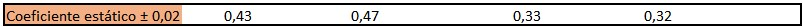
\includegraphics[width=.95\textwidth]{fotos/estatico.jpg}
        \end{figure}
    
    Como podemos comprobar, el coeficiente estático con o sin la pesa es prácticamente idéntico, variando únicamente cuando cambiamos el material de la superficie que está en contacto con el plano inclinado.
    
    \clearpage
    \subsection{Dinámico}
    Para calcular el coeficiente de fricción dinámico necesitaremos calcular la aceleración que el cuerpo alcanzó en su caída por el plano inclinado. En nuestro caso, lo hemos hecho dividiendo la mayor velocidad obtenida en el trayecto (normalmente la última) entre el tiempo total, es decir, $a = \frac{\Delta v}{\Delta t}$. El error de la aceleración entonces solo se verá afectado por la imprecisión que pueda tener el programa "Tracker", por lo que le añadiremos un error de $\pm \ 0.05\ m/s^2$ \\\\
    Sin embargo la fórmula obtenida para el coeficiente de rozamiento dinámico también incluye el ángulo, que tiene un error de $\pm \ 1^{\circ}$. Por ello habrá que hacer propagación de errores para obtener el error de cada uno de los coeficientes de rozamiento dinámicos.
    \[\triangle{\mu_d} = \sqrt{\left(\frac{\partial{\mu_d}}{\partial{a}}\right)^2 \triangle{a}^2 + \left(\frac{\partial{\mu_d}}{\partial{\theta}}\right)^2 \triangle{\theta}^2}\]
    Además sabemos que 
    \[\frac{\partial{\mu_d}}{\partial{a}} = -\frac{\sec{\theta}}{g}\]
    \[\frac{\partial{\mu_d}}{\partial{\theta}} = -\frac{1}{g}a \tan{\theta}\sec{\theta}+\tan^2{\theta} + 1\]\\
    
    Calculando el error estadístico de cada coeficiente obtenido, y añadiéndole el nominal obtenido por propagación de errores, obtenemos un error para cada coeficiente de fricción dinámico.
    \begin{figure}[h]
        \centering
        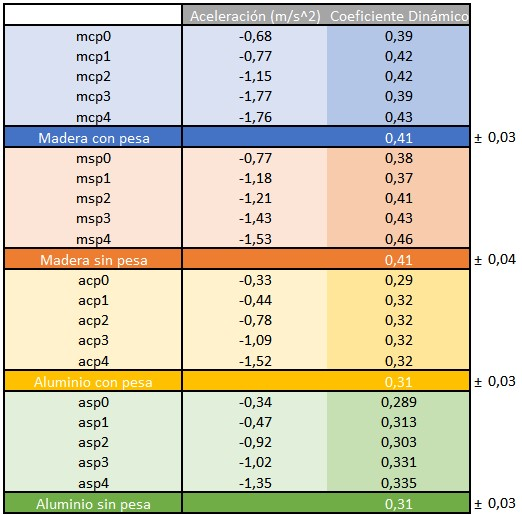
\includegraphics[width=.55\textwidth]{fotos/dinamico.jpg}
    \end{figure}\\
    Podemos comprobar como otra vez los coeficientes no cambian le pongamos o no una pesa al cuerpo, pero sí que cambian cuando hablamos de superficies de materiales distintos. El coeficiente dinámico es menor al estático lo cual cuadra con la teoría.
    \clearpage
    \subsection{Energía}
    Para calcular las energías hemos precisado del dato de la masa de los cuerpos, ya que es necesaria para calcular tanto la Energía cinética como la Energía potencial. Incluyo aquí una gráfica donde podemos ver todas las energías de una de las medidas, en particular una de las medidas de un cuerpo de madera tirado con una pesa, con el plano inclinado en $29^{\circ}$.\\
        \begin{figure}[h]
        \centering
        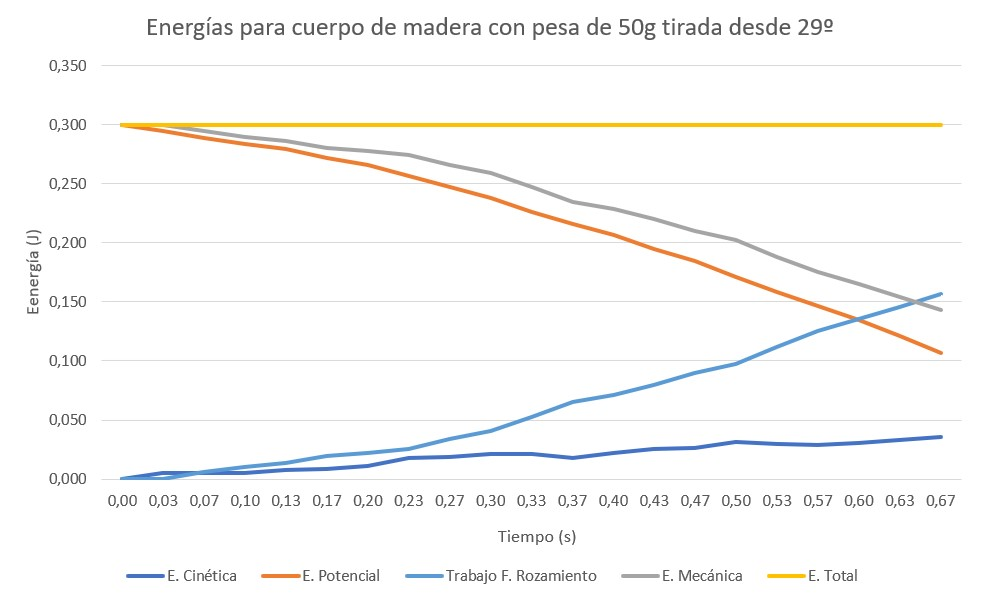
\includegraphics[width=.95\textwidth]{fotos/datos/Energías mcp2.jpg}
        \end{figure}\\
    Podemos observar como la energía potencial va poco a poco transformándose en cinética conforme avanza el tiempo, pero esta transformación no es eficiente al 100\%. Si sumamos ambas en cada instante obtendremos la Energía mecánica, que como podemos observar va claramente descendiendo a lo largo del tiempo. \\\\
    Esto nos indica que existe una fuerza disipatoria que está ejerciendo un trabajo sobre el sistema. Esta es la fuerza de rozamiento. Como podemos ver en la gráfica, cuando sumamos el trabajo realizado por la fuerza de rozamiento a la energía mecánica, obtenemos toda la energía inicial, unos $0.3 J$, que se mantienen esta vez sí, constantes en todo el recorrido del cuerpo.\\\\
    Los datos de las energías se encuentran recogidos junto con el resto de datos obtenidos y derivados del programa "Tracker" en el anexo.

%----------------------------------------------------------------------------------------
%	SECTION 5
%----------------------------------------------------------------------------------------

\pagebreak
\section{Anexo}
\subsection{Tablas de datos}
\subsubsection{Cuerpo de madera sin pesas}

\begin{figure}[h]
\centering
\hspace*{-2cm}
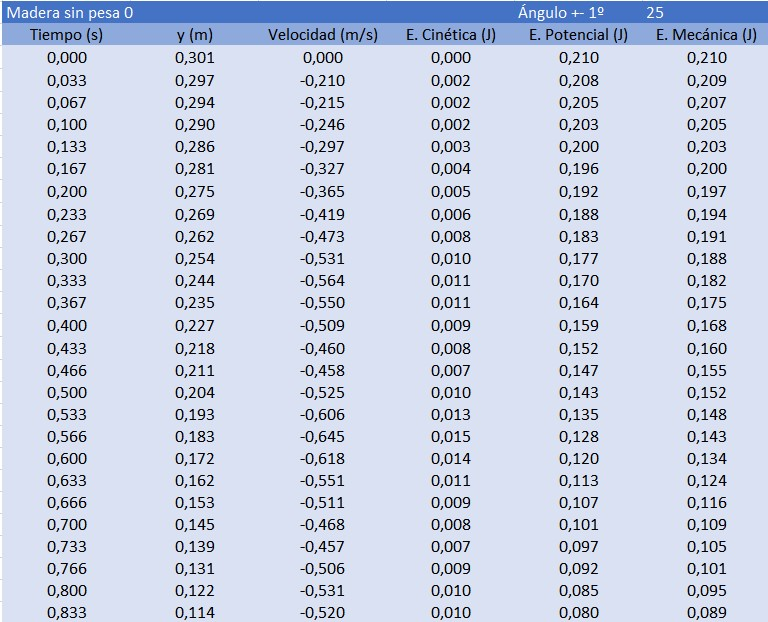
\includegraphics[width=.56\textwidth]{fotos/datos/msp0.jpg}\hfill
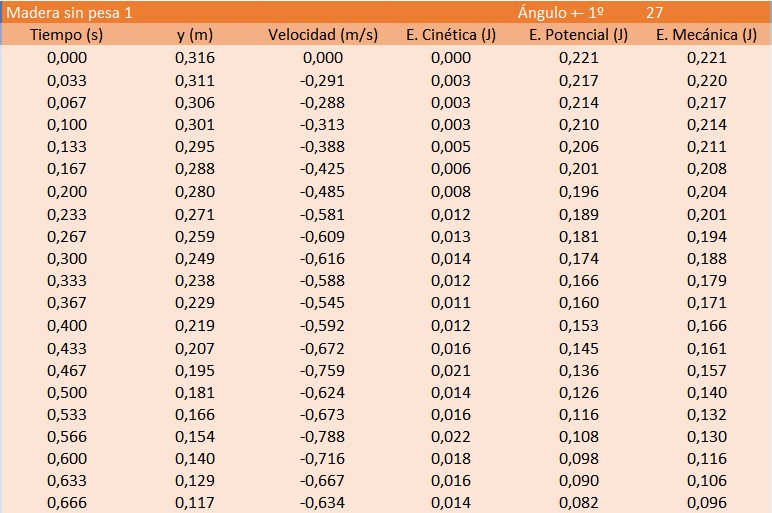
\includegraphics[width=.56\textwidth]{fotos/datos/msp1.jpg}
\hspace*{-2cm}
\end{figure}

\begin{figure}[h]
\centering
\hspace*{-2cm}
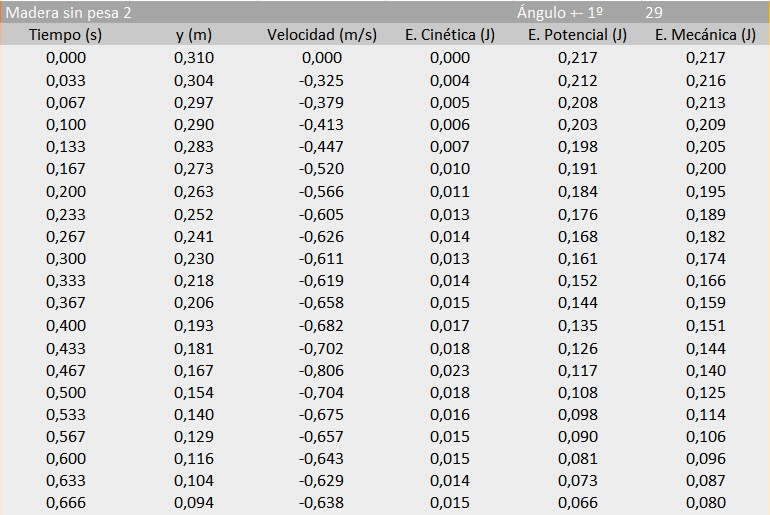
\includegraphics[width=.56\textwidth]{fotos/datos/msp2.jpg}\hfill
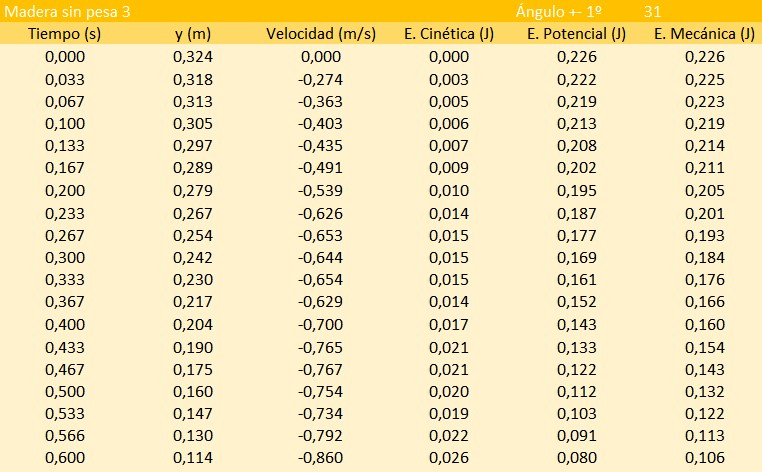
\includegraphics[width=.56\textwidth]{fotos/datos/msp3.jpg}
\hspace*{-2cm}
\end{figure}

\begin{figure}[h]
\centering
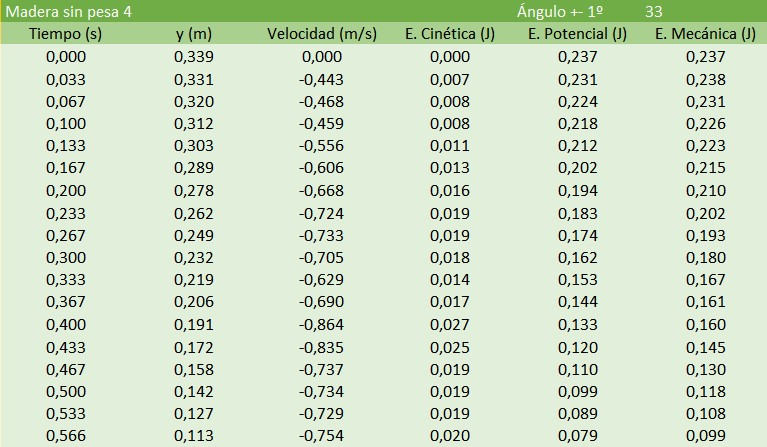
\includegraphics[width=.56\textwidth]{fotos/datos/msp4.jpg}\hfill
\end{figure}


\clearpage
\subsubsection{Cuerpo de madera con pesas}

\begin{figure}[h]
\centering
\hspace*{-2cm}
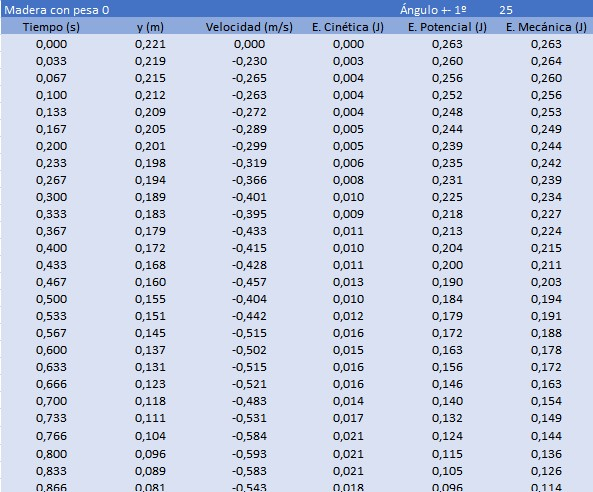
\includegraphics[width=.56\textwidth]{fotos/datos/mcp0.jpg}\hfill
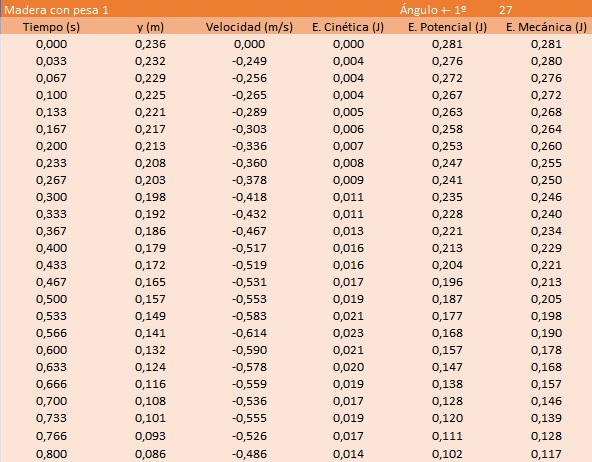
\includegraphics[width=.56\textwidth]{fotos/datos/mcp1.jpg}
\hspace*{-2cm}
\end{figure}

\begin{figure}[h]
\centering
\hspace*{-2cm}
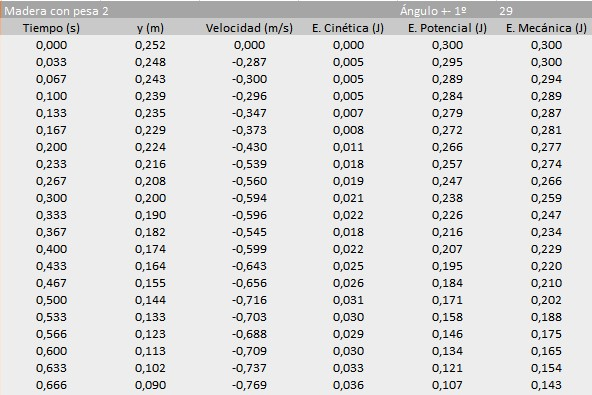
\includegraphics[width=.56\textwidth]{fotos/datos/mcp2.jpg}\hfill
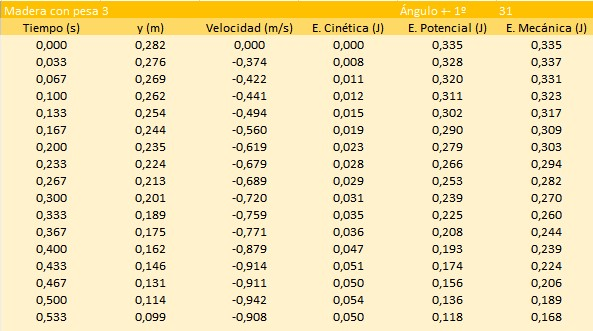
\includegraphics[width=.56\textwidth]{fotos/datos/mcp3.jpg}
\hspace*{-2cm}
\end{figure}

\begin{figure}[h]
\centering
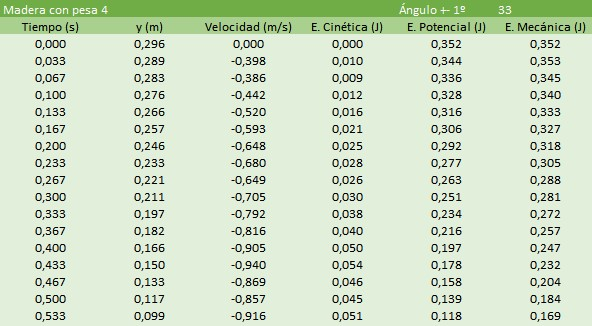
\includegraphics[width=.56\textwidth]{fotos/datos/mcp4.jpg}\hfill
\end{figure}

\clearpage
\subsubsection{Cuerpo de aluminio sin pesas}

\begin{figure}[h]
\centering
\hspace*{-2cm}
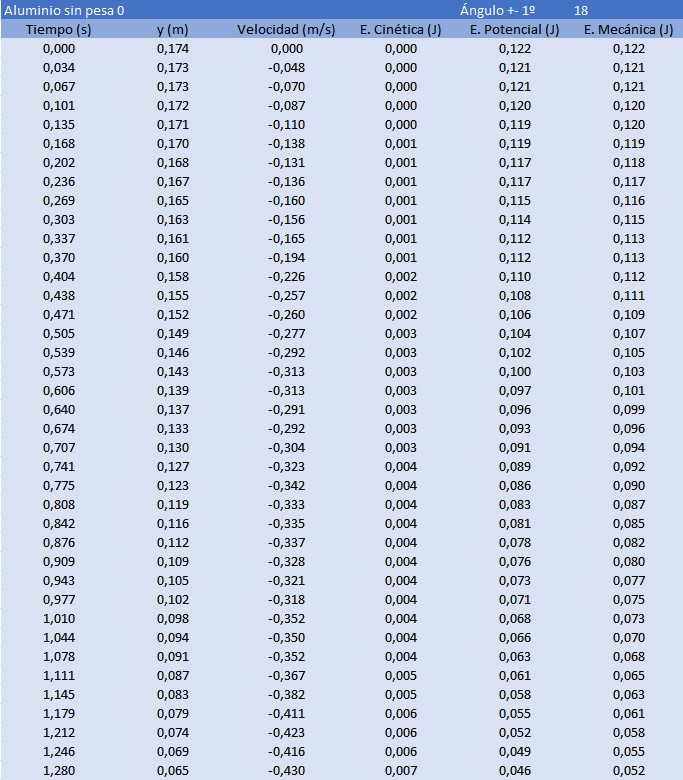
\includegraphics[width=.56\textwidth]{fotos/datos/asp0.jpg}\hfill
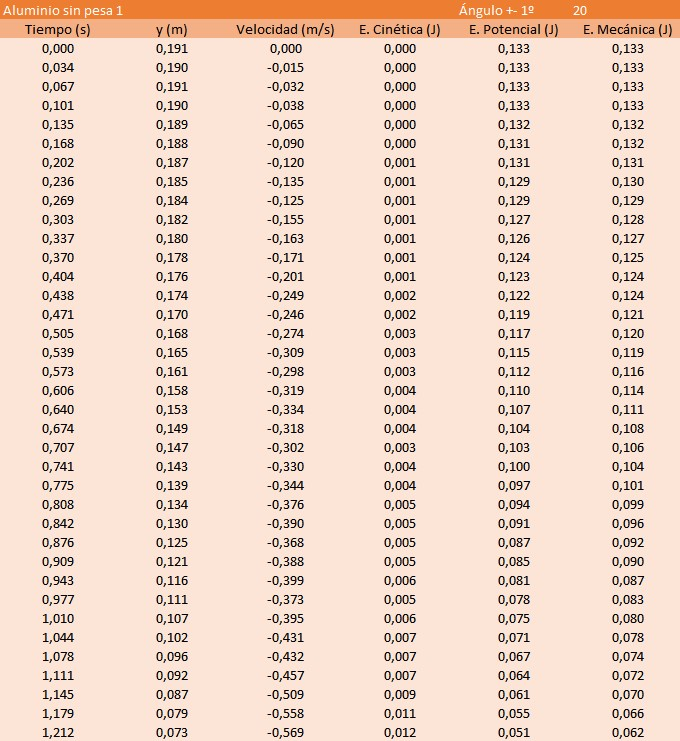
\includegraphics[width=.56\textwidth]{fotos/datos/asp1.jpg}
\hspace*{-2cm}
\end{figure}

\begin{figure}[h]
\centering
\hspace*{-2cm}
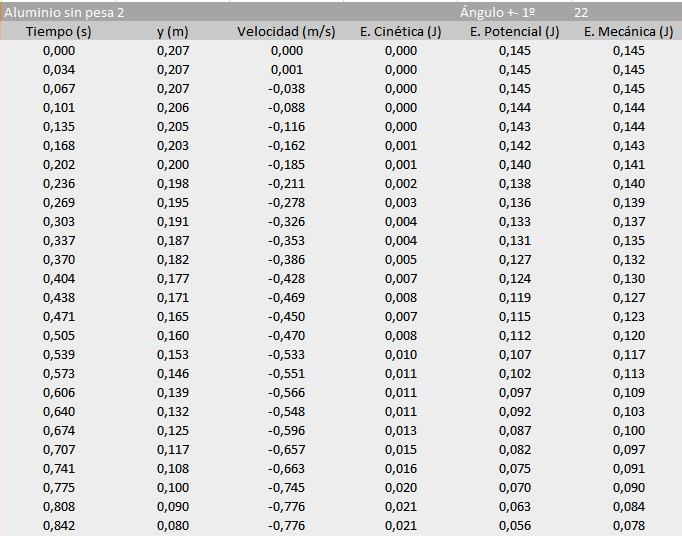
\includegraphics[width=.56\textwidth]{fotos/datos/asp2.jpg}\hfill
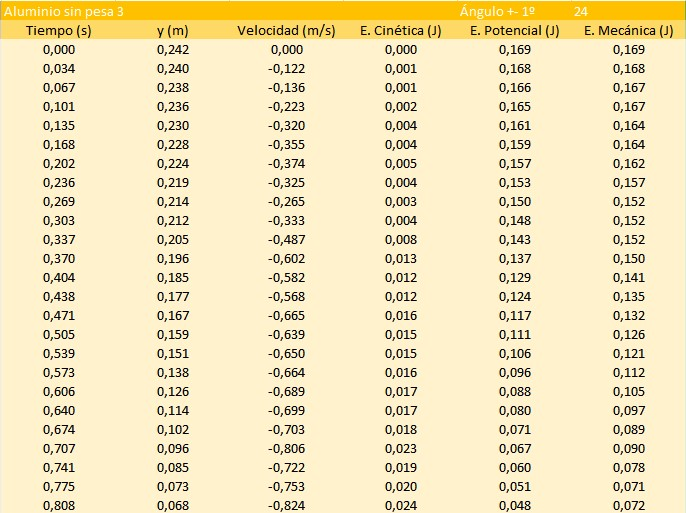
\includegraphics[width=.56\textwidth]{fotos/datos/asp3.jpg}
\hspace*{-2cm}
\end{figure}

\begin{figure}[h]
\centering
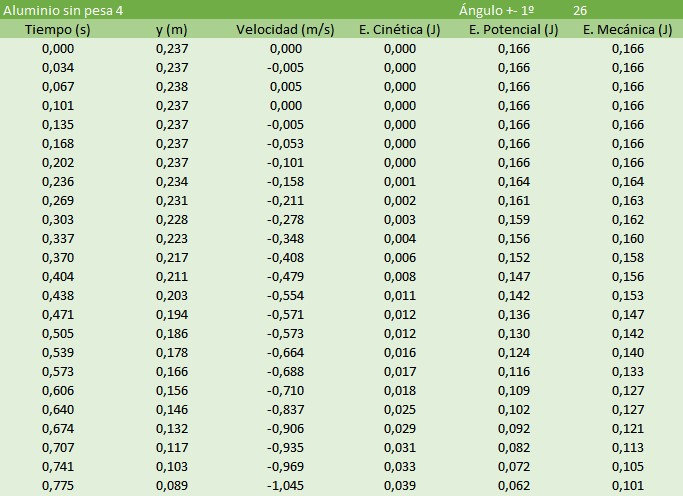
\includegraphics[width=.56\textwidth]{fotos/datos/asp4.jpg}\hfill
\end{figure}

\clearpage
\subsubsection{Cuerpo de aluminio con pesas}

\begin{figure}[h]
\centering
\hspace*{-2cm}
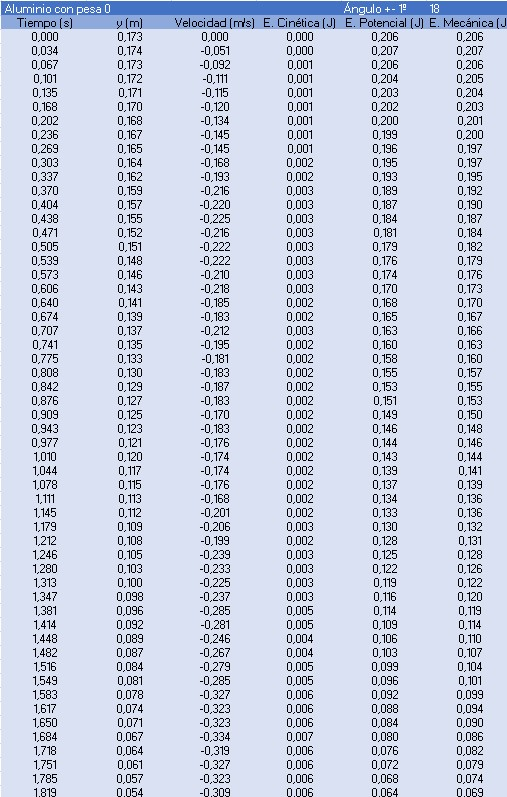
\includegraphics[width=.56\textwidth]{fotos/datos/acp0.jpg}\hfill
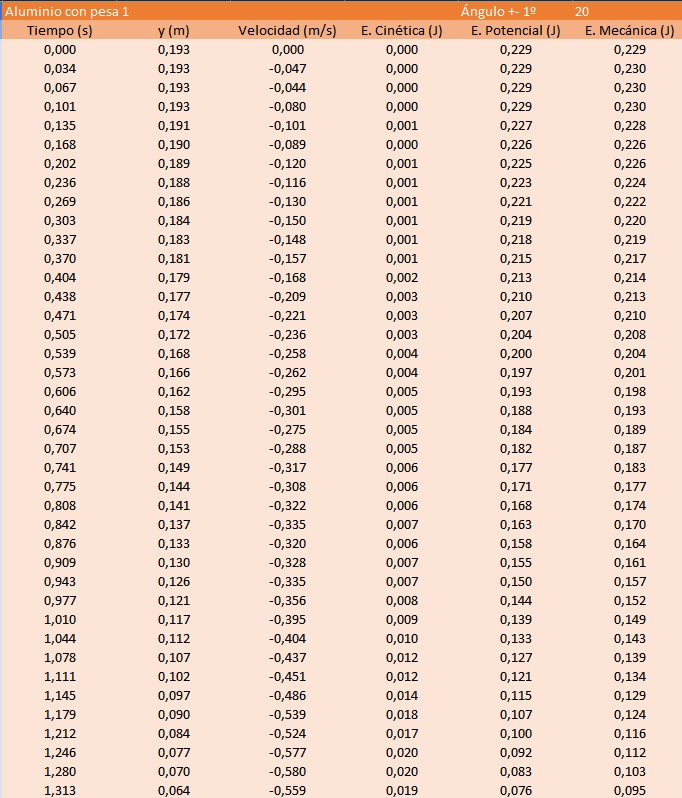
\includegraphics[width=.56\textwidth]{fotos/datos/acp1.jpg}
\hspace*{-2cm}
\end{figure}

\begin{figure}[h]
\centering
\hspace*{-2cm}
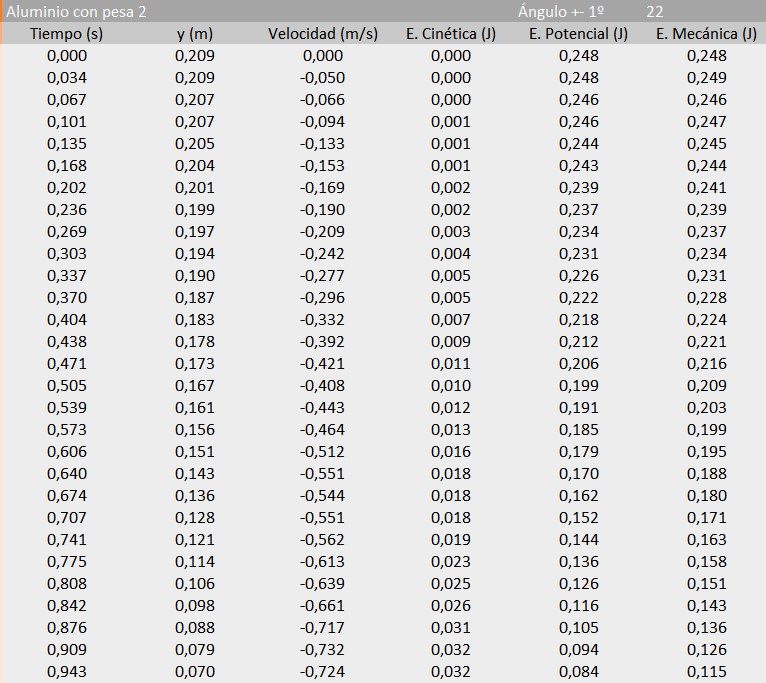
\includegraphics[width=.56\textwidth]{fotos/datos/acp2.jpg}\hfill
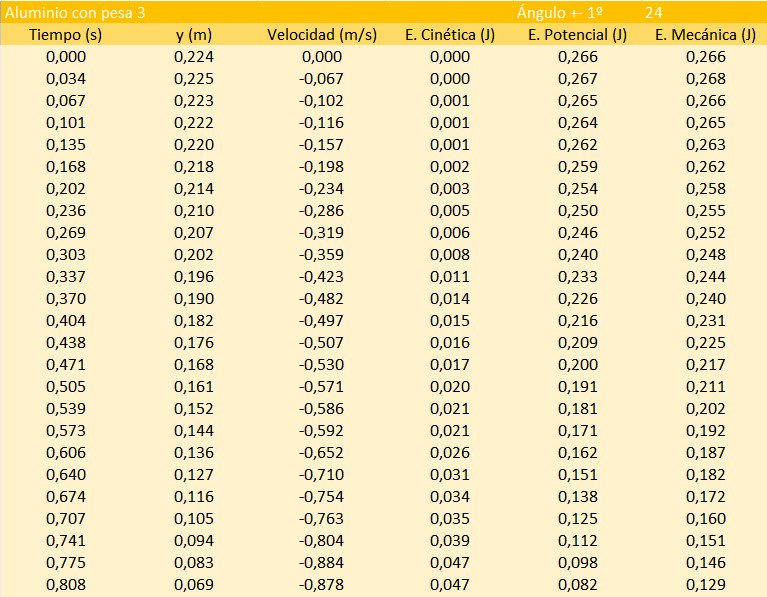
\includegraphics[width=.56\textwidth]{fotos/datos/acp3.jpg}
\hspace*{-2cm}
\end{figure}

\begin{figure}[h]
\centering
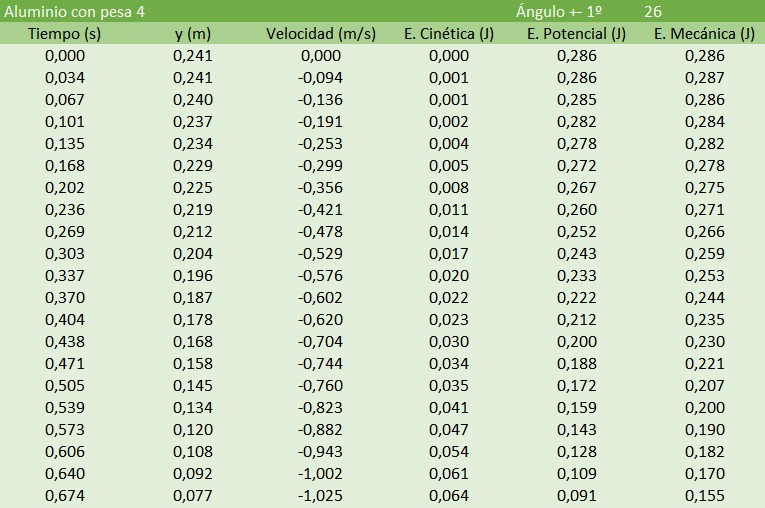
\includegraphics[width=.56\textwidth]{fotos/datos/acp4.jpg}\hfill
\end{figure}

\end{document}